% ------------------------------------------------------------
% LaTeX Template für die DHBW zum Schnellstart!
% Original: https://github.wdf.sap.corp/vtgermany/LaTeX-Template-DHBW
% ------------------------------------------------------------
% ---- Präambel mit Angaben zum Dokument
\documentclass[
	fontsize=12pt,           % Leitlinien sprechen von Schriftgröße 12.
	paper=A4,
	twoside=false,
	listof=totoc,            % Tabellen- und Abbildungsverzeichnis ins Inhaltsverzeichnis
	bibliography=totoc,      % Literaturverzeichnis ins Inhaltsverzeichnis aufnehmen
	titlepage,               % Titlepage-Umgebung anstatt \maketitle
	headsepline,             % horizontale Linie unter Kolumnentitel
	abstract,              % Überschrift einschalten, Abstract muss in {abstract}-Umgebung stehen
]{scrreprt}                  % Verwendung von KOMA-Report
\usepackage[utf8]{inputenc}  % UTF8 Encoding einschalten
\usepackage[ngerman]{babel}  % Neue deutsche Rechtschreibung
\usepackage[T1]{fontenc}     % Ausgabe von westeuropäischen Zeichen (auch Umlaute)
\usepackage{microtype}       % Trennung von Wörtern wird besser umgesetzt
\usepackage{lmodern}         % Nicht-gerasterte Schriftarten (bei MikTeX erforderlich)
\usepackage{graphicx}        % Einbinden von Grafiken erlauben
\usepackage{wrapfig}         % Grafiken fließend im Text
\usepackage{setspace}        % Zeilenabstand \singlespacing, \onehalfspaceing, \doublespacing
\setstretch{1.2}
\usepackage[
	%showframe,                % Ränder anzeigen lassen
	left=2.0cm, right=2.0cm,
	top=2.5cm,  bottom=2.5cm,
	includeheadfoot
]{geometry}                      % Seitenlayout einstellen
\usepackage{scrlayer-scrpage}    % Gestaltung von Fuß- und Kopfzeilen
\usepackage{acronym}             % Abkürzungen, Abkürzungsverzeichnis
\usepackage{titletoc}            % Anpassungen am Inhaltsverzeichnis
\contentsmargin{0.75cm}          % Abstand im Inhaltsverzeichnis zw. Punkt und Seitenzahl
\usepackage[                     % Klickbare Links (enth. auch "nameref", "url" Package)
  hidelinks,                     % Blende die "URL Boxen" aus.
  breaklinks=true                % Breche zu lange URLs am Zeilenende um
]{hyperref}
\usepackage[hypcap=true]{caption}% Anker Anpassung für Referenzen
\urlstyle{same}                  % Aktuelle Schrift auch für URLs
% Anpassung von autoref für Gleichungen (ergänzt runde Klammern) und Algorithm.
% Anstatt "Listing" kann auch z.B. "Code-Ausschnitt" verwendet werden. Dies sollte
% jedoch synchron gehalten werden mit \lstlistingname (siehe weiter unten).
\addto\extrasngerman{%
	\def\equationautorefname~#1\null{Gleichung~(#1)\null}
	\def\lstnumberautorefname{Zeile}
	\def\lstlistingautorefname{Listing}
	\def\algorithmautorefname{Algorithmus}
	% Damit einheitlich "Abschnitt 1.2[.3]" verwendet wird und nicht "Unterabschnitt 1.2.3"
	% \def\subsectionautorefname{Abschnitt}
}

% ---- Abstand verkleinern von der Überschrift 
\renewcommand*{\chapterheadstartvskip}{\vspace*{.5\baselineskip}}

% Hierdurch werden Schusterjungen und Hurenkinder vermieden, d.h. einzelne Wörter
% auf der nächsten Seite oder in einer einzigen Zeile.
% LaTeX kann diese dennoch erzeugen, falls das Layout ansonsten nicht umsetzbar ist.
% Diese Werte sind aber gute Startwerte.
\widowpenalty10000
\clubpenalty10000

% ---- Für das Quellenverzeichnis
\usepackage[
	backend = biber,                % Verweis auf biber
	language = auto,
	style = authoryear,                % Nummerierung der Quellen mit Zahlen
	sorting = true,                 % none = Sortierung nach der Erscheinung im Dokument
	sortcites = true,               % Sortiert die Quellen innerhalb eines cite-Befehls
	block = space,                  % Extra Leerzeichen zwischen Blocks
	hyperref = true,                % Links sind klickbar auch in der Quelle
	%backref = true,                % Referenz, auf den Text an die zitierte Stelle
	bibencoding = auto,
	giveninits = true,              % Vornamen werden abgekürzt
	doi=false,                      % DOI nicht anzeigen
	isbn=false,                     % ISBN nicht anzeigen
    alldates=short                  % Datum immer als DD.MM.YYYY anzeigen
]{biblatex}
\addbibresource{Inhalt/literatur.bib}
\setcounter{biburlnumpenalty}{3000}     % Umbruchgrenze für Zahlen
\setcounter{biburlucpenalty}{6000}      % Umbruchgrenze für Großbuchstaben
\setcounter{biburllcpenalty}{9000}      % Umbruchgrenze für Kleinbuchstaben
\DeclareNameAlias{default}{family-given}  % Nachname vor dem Vornamen
\AtBeginBibliography{\renewcommand{\multinamedelim}{\addslash\space
}\renewcommand{\finalnamedelim}{\multinamedelim}}  % Schrägstrich zwischen den Autorennamen
\DefineBibliographyStrings{german}{
  urlseen = {Einsichtnahme:},                      % Ändern des Titels von "besucht am"
}
\usepackage[babel,german=quotes]{csquotes}         % Deutsche Anführungszeichen + Zitate


% ---- Für Mathevorlage
\usepackage{amsmath}    % Erweiterung vom Mathe-Satz
\usepackage{amssymb}    % Lädt amsfonts und weitere Symbole
\usepackage{MnSymbol}   % Für Symbole, die in amssymb nicht enthalten sind.


% ---- Für Quellcodevorlage
\usepackage{scrhack}                    % Hack zur Verw. von listings in KOMA-Script
\usepackage{listings}                   % Darstellung von Quellcode
\usepackage{xcolor}                     % Einfache Verwendung von Farben
%% -- Eigene Farben für den Quellcode
\definecolor{JavaLila}{rgb}{0.4,0.1,0.4}
\definecolor{JavaGruen}{rgb}{0.3,0.5,0.4}
\definecolor{JavaBlau}{rgb}{0.0,0.0,1.0}
\definecolor{ABAPKeywordsBlue}{HTML}{6000ff}
\definecolor{ABAPCommentGrey}{HTML}{808080}
\definecolor{ABAPStringGreen}{HTML}{4da619}
\definecolor{PyKeywordsBlue}{HTML}{0000AC}
\definecolor{PyCommentGrey}{HTML}{808080}
\definecolor{PyStringGreen}{HTML}{008080}
% -- Farben für ABAP CDS
\definecolor{CDSString}{HTML}{FF8C00}
\definecolor{CDSKeywords}{HTML}{6000ff}
\definecolor{CDSAnnotation}{HTML}{00BFFF}
\definecolor{CDSComment}{HTML}{808080}
\definecolor{CDSFunc}{HTML}{FF0000}

% -- Default Listing-Styles

\lstset{
	% Das Paket "listings" kann kein UTF-8. Deswegen werden hier 
	% die häufigsten Zeichen definiert (ä,ö,ü,...)
	literate=%
		{á}{{\'a}}1 {é}{{\'e}}1 {í}{{\'i}}1 {ó}{{\'o}}1 {ú}{{\'u}}1
		{Á}{{\'A}}1 {É}{{\'E}}1 {Í}{{\'I}}1 {Ó}{{\'O}}1 {Ú}{{\'U}}1
		{à}{{\`a}}1 {è}{{\`e}}1 {ì}{{\`i}}1 {ò}{{\`o}}1 {ù}{{\`u}}1
		{À}{{\`A}}1 {È}{{\'E}}1 {Ì}{{\`I}}1 {Ò}{{\`O}}1 {Ù}{{\`U}}1
		{ä}{{\"a}}1 {ë}{{\"e}}1 {ï}{{\"i}}1 {ö}{{\"o}}1 {ü}{{\"u}}1
		{Ä}{{\"A}}1 {Ë}{{\"E}}1 {Ï}{{\"I}}1 {Ö}{{\"O}}1 {Ü}{{\"U}}1
		{â}{{\^a}}1 {ê}{{\^e}}1 {î}{{\^i}}1 {ô}{{\^o}}1 {û}{{\^u}}1
		{Â}{{\^A}}1 {Ê}{{\^E}}1 {Î}{{\^I}}1 {Ô}{{\^O}}1 {Û}{{\^U}}1
		{œ}{{\oe}}1 {Œ}{{\OE}}1 {æ}{{\ae}}1 {Æ}{{\AE}}1 {ß}{{\ss}}1
		{ű}{{\H{u}}}1 {Ű}{{\H{U}}}1 {ő}{{\H{o}}}1 {Ő}{{\H{O}}}1
		{ç}{{\c c}}1 {Ç}{{\c C}}1 {ø}{{\o}}1 {å}{{\r a}}1 {Å}{{\r A}}1
		{€}{{\euro}}1 {£}{{\pounds}}1 {«}{{\guillemotleft}}1
		{»}{{\guillemotright}}1 {ñ}{{\~n}}1 {Ñ}{{\~N}}1 {¿}{{?`}}1,
	breaklines=true,        % Breche lange Zeilen um 
	breakatwhitespace=true, % Wenn möglich, bei Leerzeichen umbrechen
	% Symbol für Zeilenumbruch einfügen
	prebreak=\raisebox{0ex}[0ex][0ex]{\ensuremath{\rhookswarrow}},
	postbreak=\raisebox{0ex}[0ex][0ex]{\ensuremath{\rcurvearrowse\space}},
	tabsize=4,                                 % Setze die Breite eines Tabs
	basicstyle=\ttfamily\small,                % Grundsätzlicher Schriftstyle
	columns=fixed,                             % Besseres Schriftbild
	numbers=left,                              % Nummerierung der Zeilen
	%frame=single,                             % Umrandung des Codes
	showstringspaces=false,                    % Keine Leerzeichen hervorheben
	keywordstyle=\color{blue},
	ndkeywordstyle=\bfseries\color{darkgray},
	identifierstyle=\color{black},
	commentstyle=\itshape\color{JavaGruen},   % Kommentare in eigener Farbe
	stringstyle=\color{JavaBlau},             % Strings in eigener Farbe,
	captionpos=b,                             % Bild*unter*schrift
	xleftmargin=5.0ex
}

% ---- Eigener JAVA-Style für den Quellcode
\renewcommand{\ttdefault}{pcr}               % Schriftart, welche auch fett beinhaltet
\lstdefinestyle{EigenerJavaStyle}{
	language=Java,                             % Syntax Highlighting für Java
	%frame=single,                             % Umrandung des Codes
	keywordstyle=\bfseries\color{JavaLila},    % Keywords in eigener Farbe und fett
	commentstyle=\itshape\color{JavaGruen},    % Kommentare in eigener Farbe und italic
	stringstyle=\color{JavaBlau}               % Strings in eigener Farbe
}

% ---- Eigener ABAP-Style für den Quellcode
\renewcommand{\ttdefault}{pcr}
\lstdefinestyle{EigenerABAPStyle}{
	language=[R/3 6.10]ABAP,
	morestring=[b]\|,                          % Für Pipe-Strings
	morestring=[b]\`,                          % für Backtick-Strings
	keywordstyle=\bfseries\color{ABAPKeywordsBlue},
	commentstyle=\itshape\color{ABAPCommentGrey},
	stringstyle=\color{ABAPStringGreen},
	tabsize=2,
	morekeywords={
		types,
		@data,
		as,
		lower,
		start,
		selection,
		order,
		by,
		inner,
		join,
		key,
		end,
		cast
	}
}

% ---- Eigener Python-Style für den Quellcode
\renewcommand{\ttdefault}{pcr}
\lstdefinestyle{EigenerPythonStyle}{
	language=Python,
	columns=flexible,
	keywordstyle=\bfseries\color{PyKeywordsBlue},
	commentstyle=\itshape\color{PyCommentGrey},
	stringstyle=\color{PyStringGreen}
}

%----- ABAP-CDS-View language
\lstdefinelanguage{ABAPCDS}{
	sensitive=false,
	%Keywords
	morekeywords={define,
		view,
		as,
		select,
		from,
		inner,
		join,
		on,
		key,
		case,
		when,
		then,
		else,
		end,
		true,
		false,
		cast,
		where,
		and,
		distinct,
		group,
		by,
		having,
		min,
		sum,
		max,
		count,
		avg
	},
	%Methoden
	morekeywords=[2]{
		div,
		currency\_conversion,
		dats\_days\_between,
		concat\_with\_space,
		dats\_add_days,
		dats\_is\_valid,
		dats\_add\_months,
		unit\_conversion,
		division,
		mod,
		abs,
		floor,
		ceil,
		round,
		concat,
		replace,
		substring,
		left,
		right,
		length
	},
	morecomment=[s][\color{CDSAnnotation}]{@}{:},
	morecomment=[l][\itshape\color{CDSComment}]{//},
	morecomment=[s][\itshape\color{CDSComment}]{/*}{*/},
	morestring=[b][\color{CDSString}]',
	keywordstyle=\bfseries\color{CDSKeywords},
	keywordstyle=[2]\color{CDSFunc}
}

  % Weitere Details sind ausgelagert

\usepackage{algorithm}                  % Für Algorithmen-Umgebung (ähnlich wie lstlistings Umgebung)
\usepackage{algpseudocode}              % Für Pseudocode. Füge "[noend]" hinzu, wenn du kein "endif",
                                        % etc. haben willst.

\makeatletter                           % Sorgt dafür, dass man @ in Namen verwenden kann.
                                        % Ansonsten gibt es in der nächsten Zeile einen Compilefehler.
\renewcommand{\ALG@name}{Algorithmus}   % Umbenennen von "Algorithm" im Header der Listings.
\makeatother                            % Zeichen wieder zurücksetzen
\renewcommand{\lstlistingname}{Listing} % Erlaubt das Umbenennen von "Listing" in anderen Titel.

% ---- Tabellen
\usepackage{booktabs}  % Für schönere Tabellen. Enthält neue Befehle wie \midrule
\usepackage{multirow}  % Mehrzeilige Tabellen
\usepackage{siunitx}   % Für SI Einheiten und das Ausrichten Nachkommastellen
\sisetup{locale=DE, range-phrase={~bis~}, output-decimal-marker={,}} % Damit ein Komma und kein Punkt verwendet wird.
\usepackage{xfrac} % Für siunitx Option "fraction-function=\sfrac"
\usepackage{hyperref} %teststetststsstst

% ---- Für Definitionsboxen in der Einleitung
\usepackage{amsthm}                     % Liefert die Grundlagen für Theoreme
\usepackage[framemethod=tikz]{mdframed} % Boxen für die Umrandung
%% ---- Definition für Highlight Boxen

% ---- Grundsätzliche Definition zum Style
\newtheoremstyle{defi}
  {\topsep}         % Abstand oben
  {\topsep}         % Abstand unten
  {\normalfont}     % Schrift des Bodys
  {0pt}             % Einschub der ersten Zeile
  {\bfseries}       % Darstellung von der Schrift in der Überschrift
  {:}               % Trennzeichen zwischen Überschrift und Body
  {.5em}            % Abstand nach dem Trennzeichen zum Body Text
  {\thmname{#3}}    % Name in eckigen Klammern
\theoremstyle{defi}

% ------ Definition zum Strich vor eines Texts
\newmdtheoremenv[
  hidealllines = true,       % Rahmen komplett ausblenden
  leftline = true,           % Linie links einschalten
  innertopmargin = 0pt,      % Abstand oben
  innerbottommargin = 4pt,   % Abstand unten
  innerrightmargin = 0pt,    % Abstand rechts
  linewidth = 3pt,           % Linienbreite
  linecolor = gray!40,       % Linienfarbe
]{defStrich}{Definition}     % Name der des formats "defStrich"

% ------ Definition zum Eck-Kasten um einen Text
\newmdtheoremenv[
  hidealllines = true,
  innertopmargin = 6pt,
  linecolor = gray!40,
  singleextra={              % Eck-Markierungen für die Definition
    \draw[line width=3pt,gray!50,line cap=rect] (O|-P) -- +(1cm,0pt);
    \draw[line width=3pt,gray!50,line cap=rect] (O|-P) -- +(0pt,-1cm);
    \draw[line width=3pt,gray!50,line cap=rect] (O-|P) -- +(-1cm,0pt);
    \draw[line width=3pt,gray!50,line cap=rect] (O-|P) -- +(0pt,1cm);
  }
]{defEckKasten}{Definition}  % Name der des formats "defEckKasten"  % Weitere Details sind ausgelagert

% ---- Für Todo Notes
\usepackage{todonotes}
\setlength {\marginparwidth }{2cm}      % Abstand für Todo Notizen

% ---- Zum Einbinden von PDF-Dokumenten
\usepackage{pdfpages}


% ---- Elektronische Version oder Gedruckte Version?
% ---- Unterschied: Die elektronische Version enthält keinen Platzhalter für die Unterschrift
\usepackage{ifthen}
\newboolean{e-Abgabe}
\setboolean{e-Abgabe}{false}    % false=gedruckte Fassung

% ---- Persönlichen Daten:
\newcommand{\titel}{Einführung in Transformer-Architekturen von Neuronalen Netzen}
\newcommand{\titelheader}{Transformer-Architekturen}
\newcommand{\arbeit}{Ausarbeitung Integrationsseminar}
\newcommand{\studiengang}{Wirtschaftsinformatik Software Engineering}
\newcommand{\studienjahr}{2022}
\newcommand{\autor}{Alexander Meinecke}
\newcommand{\autorReverse}{Meinecke, Alexander}
\newcommand{\verfassungsort}{Mannheim}
\newcommand{\matrikelnr}{1522347}
\newcommand{\kurs}{WWI22SEB}
\newcommand{\bearbeitungsmonat}{Dezember 2024}
\newcommand{\abgabe}{27. Januar 2025}
\newcommand{\bearbeitungszeitraum}{Dezember 2024 - 27. Januar 2025}
\newcommand{\firmaName}{SAP SE}
\newcommand{\firmaStrasse}{Dietmar-Hopp-Allee 16}
\newcommand{\firmaPlz}{69190 Walldorf, Deutschland}
\newcommand{\betreuerDhbw}{Alexander Lütke}

% ---- Metainformation für das PDF Dokument
\hypersetup{
	pdftitle    = {\titel},
	pdfsubject  = {\arbeit},
	pdfauthor   = {\autor},
	%pdfkeywords = {Keywords angeben},
	pdfcreator  = {LaTeX},
	%pdfproducer = {in der Regel pdfTeX}
}

% ---- Definition der Kopf- und Fußzeilen
\clearpairofpagestyles                          % Löschen von LaTeX Standard
\automark[section]{chapter}                     % Füllen von section und chapter
\renewcommand*{\chaptermarkformat}{}            % Entfernt die Kapitelnummer
\renewcommand*{\sectionmarkformat}{}            % Entfernt die Sectionnummer
% Angaben [für "plain"]{für "scrheadings"}
\ihead[]{\titelheader}                          % Kopfzeile links
\chead[]{}                                      % Kopfzeile mitte
\ohead[]{\rightmark}                            % Kopfzeile rechts
\ifoot[]{}                                      % Fußzeile links
\cfoot*{\sffamily\pagemark}                     % Fußzeile mitte
\ofoot[]{}                                      % Fußzeile rechts
\KOMAoptions{
   headsepline = 0.2pt,                         % Liniendicke Kopfzeile
   footsepline = false                          % Liniendicke Fußzeile
}


% ---- Hilfreiches
\newcommand{\zB}{z.\,B. }   % "z.B." mit kleinem Leeraum dazwischen (ohne wäre nicht korrekt)
\newcommand{\dash}{d.\,h. }

\newcommand{\code}[1]{\texttt{#1}} % Ist einfacher zu schreiben als ständig \texttt und erlaubt
                                   % Änderungen im Nachhinein, wenn man z.B. Inline-Code anders stylen möchte.

% ---- Silbentrennung (falls LaTeX defaults falsch / nicht gewünscht sind)
\hyphenation{HANA}         % anstatt HA-NA
\hyphenation{Graph-Script} % anstatt GraphS-cript

% ---- Beginn des Dokuments
\begin{document}
\setlength{\parindent}{0pt}              % Keine Paragraphen Einrückung.
                                         % Dafür haben wir den Abstand zwischen den Paragraphen.
\setcounter{secnumdepth}{2}              % Nummerierungstiefe fürs Inhaltsverzeichnis
\setcounter{tocdepth}{1}                 % Tiefe des Inhaltsverzeichnisses. Ggf. so anpassen,
                                         % dass das Verzeichnis auf eine Seite passt.
\sffamily                                % Serifenlose Schrift verwenden.

% ---- Vorspann
% ------ Titelseite
\singlespacing
\thispagestyle{empty}
\begin{titlepage}
\enlargethispage{4cm}

\begin{figure}           % Logo vom Ausbildungsbetrieb und der DHBW
	% \vspace*{-5mm} % Sollte dein Titel zu lang werden, kannst du mit diesem "Hack" 
	%                  den Inhalt der Seite nach oben schieben.
	\begin{minipage}{0.49\textwidth}
		\flushleft
		
\includegraphics[height=2.5cm]{Bilder/Logos/Logo_SAP.pdf} 
	\end{minipage}
	\hfill
	\begin{minipage}{0.49\textwidth}
		\flushright
		
\includegraphics[height=2.5cm]{Bilder/Logos/Logo_DHBW.pdf} 
	\end{minipage}
\end{figure} 
\vspace*{0.1cm}

\begin{center}
	\huge{\textbf{\titel}}\\[1.5cm]
	\Large{\textbf{\arbeit}}\\[0.5cm]
	\normalsize{im Rahmen der Prüfung zum\\[1ex] \textbf{Bachelor of Science (B.Sc.)}}\\[0.5cm]
	\Large{des Studienganges \studiengang}\\[1ex]
	\normalsize{an der Dualen Hochschule Baden-Württemberg Mannheim}\\[1cm]
	\normalsize{von}\\[1ex] \Large{\textbf{\autor}} \\[1cm]
	% Hinweis: Manche Dozenten möchten einen Hinweis auf den Sperrvermerk auf der Titelseite.
	% \large{{\color{red}- Sperrvermerk -}}\\[1cm]
\end{center}

\begin{center}
	\vfill
	\begin{tabular}{ll}
		Abgabedatum:                     & \abgabe \\[0.2cm]
		Bearbeitungszeitraum:            & \bearbeitungszeitraum \\[0.2cm]
		Matrikelnummer, Kurs:            & \matrikelnr , \kurs \\[0.2cm]
		Ausbildungsfirma:                & \firmaName \\
		                                 & \firmaStrasse \\
		                                 & \firmaPlz \\[0.2cm]
		
		Gutachter: 						& \betreuerDhbw \\[2cm]
	\end{tabular} 
\end{center}
\end{titlepage}
  % Titelseite
\newcounter{savepage}
\pagenumbering{Roman}                    % Römische Seitenzahlen
\onehalfspacing

% ------ Erklärung, Sperrvermerk, Abstact
\chapter*{Eidesstattliche Erklärung}
Ich versichere hiermit, dass ich meine \arbeit{} mit dem Thema:
\begin{quote}
	\textit{\titel}
\end{quote} 
gemäß § 5 der \enquote{Studien- und Prüfungsordnung DHBW Technik} vom 29. September 2017 selbstständig verfasst und keine anderen als die angegebenen Quellen und Hilfsmittel benutzt habe. Die Arbeit wurde bisher keiner anderen Prüfungsbehörde vorgelegt und auch nicht veröffentlicht.

\vspace{0.25cm}

Ich versichere zudem, dass die eingereichte elektronische Fassung mit der gedruckten Fassung übereinstimmt.

\vspace{1cm}

\verfassungsort, den \today \\[0.5cm]
\ifthenelse{\boolean{e-Abgabe}}
	{\underline{Gez. \autor}}
	{\makebox[6cm]{\hrulefill}}\\ 
\autorReverse

%\chapter*{Sperrvermerk}
Die nachfolgende Arbeit enthält vertrauliche Daten der:
\begin{quote}
	\firmaName \\
	\firmaStrasse \\
	\firmaPlz
\end{quote}

\vspace{0.5cm}

Der Inhalt dieser Arbeit darf weder als Ganzes noch in Auszügen Personen außerhalb des Prüfungsprozesses und des Evaluationsverfahrens zugänglich gemacht werden, sofern keine anderslautende Genehmigung vom Dualen Partner vorliegt.

%\renewcommand{\abstractname}{Abstract} % Veränderter Name für das Abstract
\begin{abstract}
\begin{addmargin}[1.5cm]{1.5cm}        % Erhöhte Ränder, für Abstract Look
\thispagestyle{plain}                  % Seitenzahl auf der Abstract Seite

\begin{center}
\small\textit{- English -}             % Angabe der Sprache für das Abstract
\end{center}

\vspace{0.25cm}

This is the starting point of the Abstract. For the final bachelor thesis, there must be an abstract included in your document. So, start now writing it in German and English. The abstract is a short summary with around 200 to 250 words.

\vspace{0.25cm}

Try to include in this abstract the main question of your work, the methods you used or the main results of your work.


\end{addmargin}
\end{abstract}
%\renewcommand{\abstractname}{Abstract} % Veränderter Name für das Abstract
\begin{abstract}
\begin{addmargin}[1.5cm]{1.5cm}        % Erhöhte Ränder, für Abstract Look
\thispagestyle{plain}                  % Seitenzahl auf der Abstract Seite

\begin{center}
\small\textit{- Deutsch -}             % Angabe der Sprache für das Abstract
\end{center}

\vspace{0.25cm}

Dies ist der Beginn des Abstracts. Für die finale Bachelorarbeit musst du ein Abstract in deinem Dokument mit einbauen. So, schreibe es am besten jetzt in Deutsch und Englisch. Das Abstract ist eine kurze Zusammenfassung mit ca. 200 bis 250 Wörtern.

\vspace{0.25cm}

Versuche in das Abstract folgende Punkte aufzunehmen: Fragestellung der Arbeit, methodische Vorgehensweise oder die Hauptergebnisse deiner Arbeit.


\end{addmargin}
\end{abstract}

% ------ Inhaltsverzeichnis
\singlespacing
\tableofcontents

% ------ Verzeichnisse
\renewcommand*{\chapterpagestyle}{plain}
\pagestyle{plain}
%\chapter*{Formelverzeichnis}
\addcontentsline{toc}{chapter}{Formelverzeichnis} % Hinzufügen zum Inhaltsverzeichnis 

% Definition des neuen Befehls für das Einfügen der Abkürzung der Einheit
\newcommand{\acrounit}[1]{
  \acroextra{\makebox[18mm][l]{\si[per-mode=fraction,fraction-function=\sfrac]{#1}}}
}
\begin{acronym}[dmin] % längstes Kürzel wird verw. für den Abstand zw. Kürzel u. Text

	% Alphabetisch selbst sortieren - nicht verwendete Formeln rausnehmen!
	% Allgemein: \acro{KÜRZEL}[ABKÜRZUNG]{\acrounit{SI-EINHEIT}BESCHREIBUNG}

	\acro{A}[\ensuremath{A}]{\acrounit{mm^2}Fläche}	
	\acro{D}[\ensuremath{D}]{\acrounit{mm}Werkstückdurchmesser}	
	\acro{dmin}[\ensuremath{d\textsubscript{min}}]{\acrounit{mm}kleinster Schaftdurchmesser}	
	\acro{L1}[\ensuremath{L\textsubscript{1}}]{\acrounit{mm}Länge des Werkstückes Nr. 1}	
	\acro{Fwinkel}[]{\acrounit{Grad}Freiwinkel}	
	\acro{Kwinkel}[]{\acrounit{Grad}Keilwinkel}

\end{acronym}

\listoffigures % Erzeugen des Abbildungsverzeichnisses 
\chapter*{Abkürzungsverzeichnis}
\addcontentsline{toc}{chapter}{Abkürzungsverzeichnis} % Hinzufügen zum Inhaltsverzeichnis 

\begin{acronym}[dmodel] % längstes Kürzel wird verw. für den Abstand zw. Kürzel u. Text

	% Alphabetisch selbst sortieren - nicht verwendete Kürzel rausnehmen!
	\acro{BERT}{Bidirectional Encoder Representations from Transformers}
	\acro{dmodel}{Dimension des Modells}
	\acro{GPT}{Generative Pre-trained Transformer}
	\acro{K}{Key-Matrix}
	\acro{ML}{Machine Learning}
	\acro{PE}{Positional Encoding}
	\acro{Q}{Query-Matrix}
	\acro{ReLU}{Rectified Linear Unit}
	\acro{RNN}{Recurrent Neural Network}
	\acro{T5}{Text-to-Text Transfer Transformer}
	\acro{V}{Value-Matrix}

\end{acronym}
           
%\listoftables                           % Erzeugen des Tabellenverzeichnisses
%\renewcommand{\lstlistlistingname}{Quellcodeverzeichnis}
%\lstlistoflistings                      % Erzeugen des Listenverzeichnisses
\setcounter{savepage}{\value{page}}


% ---- Inhalt der Arbeit
\cleardoublepage
\pagenumbering{arabic}                  % Arabische Seitenzahlen für den Hauptteil
\setlength{\parskip}{0.5\baselineskip}  % Abstand zwischen Absätzen
\rmfamily
\renewcommand*{\chapterpagestyle}{scrheadings}
\pagestyle{scrheadings}
\onehalfspacing
\chapter{Einleitung}

Transformer-Architekturen haben die Landschaft der neuronalen Netze revolutioniert und neue Maßstäbe in Bereichen wie maschineller Übersetzung, Textgenerierung und Sprachverarbeitung gesetzt.  

\section{Motivation und Ziel der Arbeit}

Der Grund, warum Transformer im Bereich der Textanalyse und -verarbeitung so gut sind, ist ihre einzigartige Architektur.  
Sie sind dadurch viel effizienter, schneller und erzielen auch bessere Ergebnisse als alternative Ansätze.  
Die klassische Transformer-Architektur wurde 2017 in einem Paper mit dem Titel \enquote{Attention is All You Need} vorgestellt (vgl. \cite{attention}).  
Diese Grundlagen zu verstehen, ermöglicht es auch, bekannte Modelle wie BERT, GPT oder T5 zu verstehen.  
Ziel dieser Arbeit ist es, dem Leser ohne viel Vorwissen die klassischen Konzepte der Transformer-Architektur im Kontext der Textverarbeitung zu verdeutlichen.  

\section{Aufbau der Arbeit}

Zunächst werden im folgenden Kapitel dem Leser Grundlagen von neuronalen Netzen vermittelt, die helfen, die Notwendigkeit von Transformern in der Geschichte von neuronalen Netzen zu verstehen.  
Anschließend wird sich ein Kapitel mit dem Kernkonzept von Transformern beschäftigen, das dem Model hilft, den Kontext von Texten schnell und effizient zu analysieren.  
Dies wird zusätzlich mit einem praktischen Beispiel erläutert.  
Darauf folgt die Erklärung der Transformer-Architektur und ihrer Komponenten im Detail.  
Am Ende folgt noch ein Fazit, das noch einmal die wichtigsten Aspekte zusammenfasst.  

\chapter{Grundlagen}

Um zu verstehen, wie Transformer funktionieren, muss zunächst ein kurzer Überblick über neuronale Netze gegeben werden.  

\section{Neuronale Netze}

Neuronale Netze sind ein Teilgebiet des maschinellen Lernens.
Sie sind trainierbar und können die gesammelten Erfahrungen auf neue Daten anwenden.  
Neuronale Netze orientieren sich an der Struktur des menschlichen Gehirns (vgl. \cite[S. 14]{Kinnebrock.2018}).  
Sie bestehen aus mehreren Schichten von Neuronen (vgl. \cite[S. 25]{Kinnebrock.2018}).  

Es gibt dabei eine Eingabe- und Ausgabeschicht sowie mehrere versteckte Schichten, in denen die eigentliche Verarbeitung stattfindet.  
Jedes Neuron verarbeitet seine eigenen Daten, gewichtet sie und addiert sie mit den Ergebnissen der vorherigen Schicht.  
Dieses Ergebnis wird dann an die Aktivierungsfunktion weitergegeben, um die nächsten verbundenen Neuronen anzusteuern.  
Diese Funktion bestimmt, ob das Neuron \enquote{feuert} und das Signal weitergeleitet wird (vgl. \cite[S. 14]{Kinnebrock.2018}).  

Über die Jahre haben sich neuronale Netze besonders für Anwendungen wie Bildanalysen als äußerst effektiv erwiesen (vgl. \cite[S. 16]{paass.2020}).  
Doch ein Problem war lange die Textanalyse und -verarbeitung (vgl. \cite[S. 22]{paass.2020}).
Hier besteht die Herausforderung darin, dass Informationen nicht wie bei einem Bild simultan erfasst werden können.  
Um den Sinn eines Satzes zu verstehen, muss der Inhalt schrittweise verarbeitet werden.  

\section{Neuronale Netze für Textverarbeitung}

Für Textanalysen, Übersetzungen oder Zusammenfassungen wurden lange Zeit Recurrent Neural Networks (RNNs) verwendet (siehe Abb. \ref{fig:rnn}).  
RNNs analysieren einen Text sequentiell und verknüpfen jedes Wort mit dem Kontext aus dem vorhergehenden Wort (vgl. \cite[S. 2]{attention}).


\begin{figure}[ht]
	\centering
	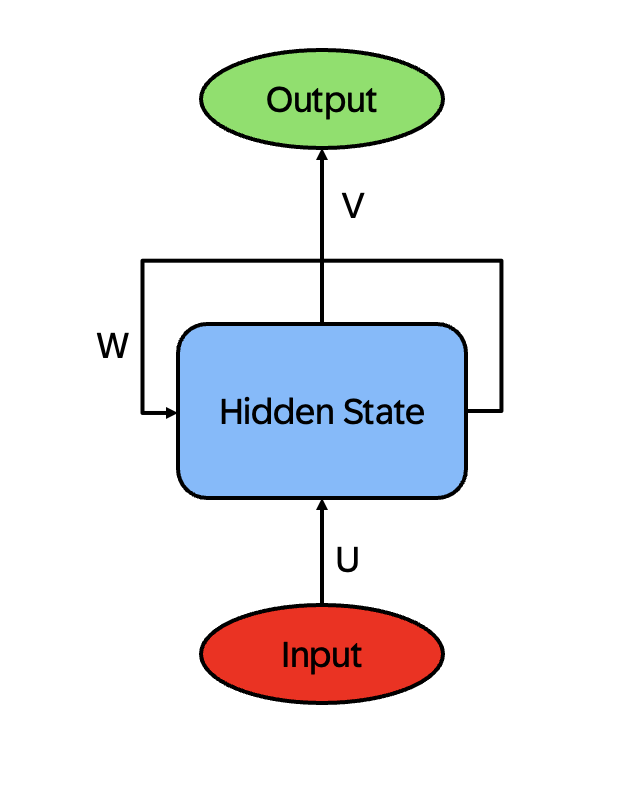
\includegraphics[width=0.3\textwidth]{Bilder/RNN.png}
	\caption{RNN als Vorgänger zum Transformer}
	\label{fig:rnn}
\end{figure}

Doch RNNs haben Schwächen (vgl. \cite[S. 2]{attention}) (vgl. \cite[S. 208]{paass.2020}).
Sie haben Schwierigkeiten, den Kontext von größeren Texten vollständig zu erfassen.  
Außerdem ist die sequentielle Verarbeitung ineffizient und schlecht auf moderne Hardware optimiert, die auf Parallelverarbeitung ausgelegt ist.  

Um diese Probleme zu lösen, wurde eine neue Art neuronaler Netze entwickelt: die Transformer.

\chapter{Die Funktionsweise von Self-Attention}

Transformer arbeiten mit dem zentralen Baustein Self-Attention.
Self-Attention ist ein Algorithmus der letztendlich Zusammenhänge zwischen Wörtern z.B. in einem Text aufzeigt.
Wörter werden in Form von Tokens verarbeitet, die ganze Wörter oder Wortteile sein können.
Jeder Token ist einzigartig und wird zunächst nur durch eine natürliche Zahl repräsentiert.

\section{Generierung von Embeddings}

Grundlage jedes Attention-Zyklus sind Eingabe-Tokens.  
Um die mathematische Vorgehensweise besser zu veranschaulichen, wird im Folgenden der Satz \enquote{Ich sitze auf der Bank} als Beispiel verarbeitet.
Dafür wird auf das Transformer-Model \enquote{BERT} zurückgegriffen.
Jedes dieser Wörter ist ein eigener Token, der vor der Eingabe in den Attention-Zyklus vom Transformer übersetzt wird:
[\enquote{[CLS]}, \enquote{ich}, \enquote{sit}, \enquote{##ze}, \enquote{auf}, \enquote{der}, \enquote{bank}, \enquote{[SEP]}].  
\enquote{[CLS]} ist ein Klassifizierungstoken, der am Anfang jeder Eingabesequenz eingefügt wird.
\enquote{[SEP]} trennt verschiedene Teile dieser Eingabesequenz.
Diese Tokens sehen für das Model wie folgt aus: [101, 22564, 4133, 4371, 21200, 4315, 2924, 102].
Die Herausforderung für den Transformer besteht darin, aus dem Kontext der anderen Tokens zu erkennen, ob \enquote{Bank} eine Sitzbank oder das Finanzinstitut Bank bedeutet.

Jeder Token bildet ein Schlüssel-Werte-Paar.
Der korrespondierende Wert hinter einem Token ist ein Vektor, der die Bedeutung eines Tokens hinsichtlich mehrerer Dimensionen beschreibt.  
Diese Vektoren sind aus Trainingsdaten des Transformer-Modells entstanden.

Im ersten Schritt des Attention-Zyklus wird jeder Token in den dazugehörigen Vektor übersetzt.  
Diese Vektoren werden in der Matrix $\mathbf{X}$ gespeichert, wobei jede Zeile einen Token repräsentiert.  
Dieser Prozess wird als \textbf{Embedding} bezeichnet.  
Jeder dieser Vektoren hat gemäß der Literatur mindestens 512 Dimensionen.  
Es wird von einem \( d_{\text{model}} = 512 \) gesprochen.  
Es gilt: Je größer das \( d_{\text{model}} \), desto präziser kann der Transformer die Zusammenhänge zwischen Tokens erkennen.

Wenn sich Tokens im Vektorraum nahe liegen, haben sie eher Gemeinsamkeiten im Vergleich zu Tokens, die weit auseinander liegen.  
Angenommen, es gäbe nur ein \( d_{\text{model}} = 2 \) für jeden Token, könnten diese zwei Dimensionen als Koordinaten genutzt werden, um Zusammenhänge visuell als Cluster in einem Koordinatensystem darzustellen.  
Hier wären beispielsweise die Tokens \enquote{Hund} und \enquote{Katze} nah beieinander.

Für das oben genannte Beispiel \enquote{Ich sitze auf der Bank} nehmen wir der Übersichtlichkeit halber ein \( d_{\text{model}} = 4 \).  
So ergibt sich eine Embedding-Matrix $\mathbf{X}$ mit 5 Zeilen für 5 Tokens und 4 Spalten für jeweils 4 Dimensionen:

\[
\centering
\mathbf{X} =
\begin{bmatrix}
0.4 & 0.8 & 1.5 & 1.6 \\
3.2 & 0.4 & 0.7 & 0.2 \\
0.6 & 0.9 & 1.2 & 0.5 \\
2.1 & 0.5 & 2.0 & 0.2 \\
0.7 & 2.4 & 0.1 & 0.9
\end{bmatrix}
\]

\section{Lineare Transformation in Query-, Key- und Value-Matrizen}

Die Embedding-Matrix $\mathbf{X}$ wird durch drei Gewichtungsmatrizen $\mathbf{W_Q}$, $\mathbf{W_K}$ und $\mathbf{W_V}$, die aus dem Training des Transformer-Modells stammen, in drei neue Matrizen transformiert:

\[
\mathbf{Q} = \mathbf{X} \cdot \mathbf{W_Q}
\]
\[
\mathbf{K} = \mathbf{X} \cdot \mathbf{W_K}
\]
\[
\mathbf{V} = \mathbf{X} \cdot \mathbf{W_V}
\]

Die drei Matrizen haben im Attention-Zyklus umgangssprachlich formuliert folgende Funktionen:

\begin{itemize}
    \item \textbf{Query-Matrix (\(\mathbf{Q}\))}: Was fragt ein Token?
    \item \textbf{Key-Matrix (\(\mathbf{K}\))}: Welche Tokens im Kontext antworten am besten auf die Frage?
    \item \textbf{Value-Matrix (\(\mathbf{V}\))}: Erlernten Informationen über ein Token.
\end{itemize}

Im Beispiel könnten die jeweiligen Zeilen der Matrizen \(\mathbf{Q}\), \(\mathbf{K}\), \(\mathbf{V}\) für das Token \enquote{Bank} folgendermaßen aussehen:

\[
\begin{aligned}
\math{Q}_{\text{Bank}} &= [1.0, 0.7, 0.9, 1.1], \quad 
\math{K}_{\text{Bank}} &= [0.8, 0.6, 1.0, 0.9], \quad 
\math{V}_{\text{Bank}} &= [0.9, 0.5, 0.7, 1.0]
\end{aligned}
\]

\section{Berechnung und Einbeziehung von Attention-Scores}

Um die Relevanz zwischen \(\math{Q}\) und \(\math{K}\) zu messen, wird jeweils das Skalarprodukt zwischen jedem Tokenvektor von \(\math{Q}_{\text{T}}\) und \(\math{K}_{\text{T}}\) gebildet.  
Also im Beispiel wird unter anderem der Tokenvektor \(\math{Q}_{\text{Bank}}\) mit jedem Tokenvektor \(\math{K}_{\text{T}}\) multipliziert.

\[
\begin{aligned}
\text{Score}_{\text{Bank,Ich}} &= [1.0, 0.7, 0.9, 1.1] \cdot [0.4, 0.5, 0.1, 0.3] \\
&= 0.4 + 0.35 + 0.09 + 0.33 &= 1.17 \\
\text{Score}_{\text{Bank,Sitze}} &= [1.0, 0.7, 0.9, 1.1] \cdot [0.9, 0.8, 0.75, 0.8] \\
&= 0.9 + 0.56 + 0.675 + 0.88 &= 3.015 \\
\vdots \\
\text{Scores}_{\text{Bank}} &= [1.17, 3.015, 2.92, 1.12, 2.98]
\end{aligned}
\]


Die berechneten Attentionscores müssen noch zwei Verfahren unterlaufen.
Einmal ist das die Fokussierung und Normalisierung der Attentionscores mit der \textbf{Softmax-Funktion}.
\[
\text{Softmax}(x_i) = \frac{\exp(x_i)}{\sum_{j} \exp(x_j)}
\]

\(\math{x}\) ist der jeweilige aktuell zu betrachtende Attention-Score-Vektor.  
\(i\) ist der aktuell zu betrachtende Werteindex in diesem Vektor.  
\(j\) ist die Gesamtanzahl an Werten in \(\math{x}\).

Bei der \textbf{Fokussierung} werden höhere Attention-Score-Werte zwischen \(\mathbf{Q}\) und \(\mathbf{K}\) exponentiell bevorzugt.  
Analog dazu werden niedrigere Attention-Score-Werte exponentiell nach unten bewertet.  
Bei der zweiten Aufgabe der Softmax-Funktion, der \textbf{Normalisierung}, werden die Attention-Score-Werte pro Score-Vektor in Wahrscheinlichkeiten zwischen \(0\) und \(1\) transformiert, wobei die Summe jedes Attention-Score-Vektors immer \(1\) ist.

Damit die Softmax-Funktion aber optimal funktionieren kann, müssen die Werte in den Attention-Score-Vektoren erst einmal dimensioniert werden.
Bei geläufigen Transformermodellen wird wie oben beschrieben, ein \( d_{\text{model}} \) von mindestens 512 verwendet.
Durch diese großen Dimensionen entehen bei der Berechnung von den Attention-Scores durch die Aufsummierung bei der Bildung des Skalarprodukte sehr große Werte.
Diese großen Werte sorgen dafür, dass die Softmax-Funktion viele Q-K-Beziehungen sehr hoch bewertet und so der Transformer nicht sich auf die tatsächlich vielversprechenden Verbindungen konzentrieren kann und so die Weiterverarbeitung ungenau wird.
Diese Werte fallen bei dem oben gerechneten Beispiel nicht auf, da hier nur mit einem \( d_{\text{model}} \) von vier gerechnet wird.

Um hohe Attention-Score-Werte zu normalisieren, werden die Attention-Score-Vektor-Werte durch \( \sqrt{d_{\text{model}}} \) geteilt und so für die Softmax-Funktion in einen stabilen Bereich gebracht. \\
So kann ein Transformer auch kleine Relevanzunterschiede in der Token-Beziehung berücksichtigen.
Hier beispielsweise für das Attention-Score-Array von \enquote{Bank}:

\[
\frac{\text{Scores}_{\text{Bank}}}{\sqrt{4}} = [0.585, 1.5075, 1.46, 0.56, 1.49]
\]

\[
\text{Softmax}\left(\frac{\text{Scores}_{\text{Bank}}}{\sqrt{4}}\right) = [0.107, 0.269, 0.256, 0.104, 0.264]
\]

Damit diese nun umgewandelten Attention-Score-Wahrscheinlichkeiten in den weiteren Verarbeitungsschritten berücksichtigt werden können, werden sie mit der \( V \)-Matrix multipliziert. 
Das zeigt dem Modell, zu wie viel Prozent der erlernten Informationen zu einem Token im nächsten Schritt einfließen.
Insgesamt sieht das Verfahren folgendermaßen aus:

\[
\text{Attention}(Q, K, V) = \operatorname{Softmax}\left(\frac{QK^T}{\sqrt{d_{\text{model}}}}\right) V
\]

%Also werden die finalen die Informationen für Bank \math{V}_{\text{Bank}} folgendermaßen gewichtet:

%\[
%\math{Z}_{\text{Bank}} = [0.107, 0.269, 0.256, 0.104, 0.264] \cdot [0.9, 0.5, 0.7, 1.0] = [0.9, 0.5, 0.7, 1.0]
%\]
\chapter{Transformer-Architektur im Detail}

Im ursprünglichen Werk \textit{Attention Is All You Need} \todo{cite}, in dem das grundlegende Transformer-Modell vorgestellt wurde, besteht ein Transformer aus zwei Hauptkomponenten: 
dem Encoder und dem Decoder.

Encoder und Decoder verarbeiten Text in Form von Tokens, die ganze Wörter oder Wortteile sein können. 
Jeder Token ist für den Transformer einzigartig und wird zunächst nur durch eine natürliche Zahl repräsentiert.

Der \textbf{Encoder} übersetzt die Eingabewörter in eine abstrahierte Repräsentation.  
Ziel ist es hierbei, die semantischen und syntaktischen Informationen des Textes zu extrahieren und zu kodieren.  
Die andere Komponente, der \textbf{Decoder}, nutzt diese Repräsentation, um passende Outputs zu generieren. 
Dabei berechnet er in jeder Iteration den nächsten am besten passenden Token, der zum Output hinzugefügt werden soll. 
Hierbei bezieht er auch den zuletzt generierten Token in die Berechnung des nächsten Tokens ein.

Grundlage für sowohl den Encoder als auch den Decoder ist das Self-Attention-Konzept, das im folgenden Abschnitt näher erläutert wird.


\chapter{Transformer in der Praxis}
\chapter{Fazit}

% ---- Literaturverzeichnis
\cleardoublepage
\renewcommand*{\chapterpagestyle}{plain}
\pagestyle{plain}
\pagenumbering{Roman}                   % Römische Seitenzahlen
\setcounter{page}{\numexpr\value{savepage}+1}
\printbibliography[title=Literaturverzeichnis]

% ---- Anhang
\appendix
%\clearpage
%\pagenumbering{Roman}  % römische Seitenzahlen für Anhang

\newpage
\end{document}